\documentclass[twoside]{book}

% Packages required by doxygen
\usepackage{fixltx2e}
\usepackage{calc}
\usepackage{doxygen}
\usepackage[export]{adjustbox} % also loads graphicx
\usepackage{graphicx}
\usepackage[utf8]{inputenc}
\usepackage{makeidx}
\usepackage{multicol}
\usepackage{multirow}
\PassOptionsToPackage{warn}{textcomp}
\usepackage{textcomp}
\usepackage[nointegrals]{wasysym}
\usepackage[table]{xcolor}

% Font selection
\usepackage[T1]{fontenc}
\usepackage[scaled=.90]{helvet}
\usepackage{courier}
\usepackage{amssymb}
\usepackage{sectsty}
\renewcommand{\familydefault}{\sfdefault}
\allsectionsfont{%
  \fontseries{bc}\selectfont%
  \color{darkgray}%
}
\renewcommand{\DoxyLabelFont}{%
  \fontseries{bc}\selectfont%
  \color{darkgray}%
}
\newcommand{\+}{\discretionary{\mbox{\scriptsize$\hookleftarrow$}}{}{}}

% Page & text layout
\usepackage{geometry}
\geometry{%
  a4paper,%
  top=2.5cm,%
  bottom=2.5cm,%
  left=2.5cm,%
  right=2.5cm%
}
\tolerance=750
\hfuzz=15pt
\hbadness=750
\setlength{\emergencystretch}{15pt}
\setlength{\parindent}{0cm}
\setlength{\parskip}{3ex plus 2ex minus 2ex}
\makeatletter
\renewcommand{\paragraph}{%
  \@startsection{paragraph}{4}{0ex}{-1.0ex}{1.0ex}{%
    \normalfont\normalsize\bfseries\SS@parafont%
  }%
}
\renewcommand{\subparagraph}{%
  \@startsection{subparagraph}{5}{0ex}{-1.0ex}{1.0ex}{%
    \normalfont\normalsize\bfseries\SS@subparafont%
  }%
}
\makeatother

% Headers & footers
\usepackage{fancyhdr}
\pagestyle{fancyplain}
\fancyhead[LE]{\fancyplain{}{\bfseries\thepage}}
\fancyhead[CE]{\fancyplain{}{}}
\fancyhead[RE]{\fancyplain{}{\bfseries\leftmark}}
\fancyhead[LO]{\fancyplain{}{\bfseries\rightmark}}
\fancyhead[CO]{\fancyplain{}{}}
\fancyhead[RO]{\fancyplain{}{\bfseries\thepage}}
\fancyfoot[LE]{\fancyplain{}{}}
\fancyfoot[CE]{\fancyplain{}{}}
\fancyfoot[RE]{\fancyplain{}{\bfseries\scriptsize Generated by Doxygen }}
\fancyfoot[LO]{\fancyplain{}{\bfseries\scriptsize Generated by Doxygen }}
\fancyfoot[CO]{\fancyplain{}{}}
\fancyfoot[RO]{\fancyplain{}{}}
\renewcommand{\footrulewidth}{0.4pt}
\renewcommand{\chaptermark}[1]{%
  \markboth{#1}{}%
}
\renewcommand{\sectionmark}[1]{%
  \markright{\thesection\ #1}%
}

% Indices & bibliography
\usepackage{natbib}
\usepackage[titles]{tocloft}
\setcounter{tocdepth}{3}
\setcounter{secnumdepth}{5}
\makeindex

% Hyperlinks (required, but should be loaded last)
\usepackage{ifpdf}
\ifpdf
  \usepackage[pdftex,pagebackref=true]{hyperref}
\else
  \usepackage[ps2pdf,pagebackref=true]{hyperref}
\fi
\hypersetup{%
  colorlinks=true,%
  linkcolor=blue,%
  citecolor=blue,%
  unicode%
}

% Custom commands
\newcommand{\clearemptydoublepage}{%
  \newpage{\pagestyle{empty}\cleardoublepage}%
}

\usepackage{caption}
\captionsetup{labelsep=space,justification=centering,font={bf},singlelinecheck=off,skip=4pt,position=top}

%===== C O N T E N T S =====

\begin{document}

% Titlepage & ToC
\hypersetup{pageanchor=false,
             bookmarksnumbered=true,
             pdfencoding=unicode
            }
\pagenumbering{roman}
\begin{titlepage}
\vspace*{7cm}
\begin{center}%
{\Large My Project }\\
\vspace*{1cm}
{\large Generated by Doxygen 1.8.11}\\
\end{center}
\end{titlepage}
\clearemptydoublepage
\tableofcontents
\clearemptydoublepage
\pagenumbering{arabic}
\hypersetup{pageanchor=true}

%--- Begin generated contents ---
\chapter{Hierarchical Index}
\section{Class Hierarchy}
This inheritance list is sorted roughly, but not completely, alphabetically\+:\begin{DoxyCompactList}
\item \contentsline{section}{Equipamento}{\pageref{class_equipamento}}{}
\begin{DoxyCompactList}
\item \contentsline{section}{Motor}{\pageref{class_motor}}{}
\end{DoxyCompactList}
\end{DoxyCompactList}

\chapter{Class Index}
\section{Class List}
Here are the classes, structs, unions and interfaces with brief descriptions\+:\begin{DoxyCompactList}
\item\contentsline{section}{\hyperlink{class_equipamento}{Equipamento} }{\pageref{class_equipamento}}{}
\item\contentsline{section}{\hyperlink{class_motor}{Motor} }{\pageref{class_motor}}{}
\end{DoxyCompactList}

\chapter{Class Documentation}
\hypertarget{class_equipamento}{}\section{Equipamento Class Reference}
\label{class_equipamento}\index{Equipamento@{Equipamento}}


Inheritance diagram for Equipamento\+:
\nopagebreak
\begin{figure}[H]
\begin{center}
\leavevmode
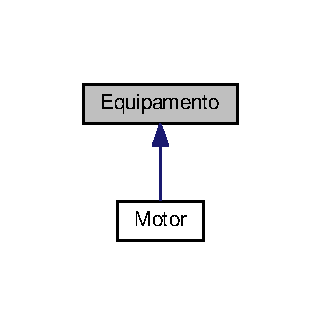
\includegraphics[width=154pt]{class_equipamento__inherit__graph}
\end{center}
\end{figure}
\subsection*{Public Member Functions}
\begin{DoxyCompactItemize}
\item 
{\bfseries Equipamento} (int a)\hypertarget{class_equipamento_a1553c92f3915ebbe7aee549d2862e440}{}\label{class_equipamento_a1553c92f3915ebbe7aee549d2862e440}

\item 
void {\bfseries set\+Nome} (const char $\ast$\+\_\+nome)\hypertarget{class_equipamento_a76c33c8f7b2c89846ce61cdbca58bbf8}{}\label{class_equipamento_a76c33c8f7b2c89846ce61cdbca58bbf8}

\item 
void {\bfseries set\+Fabricante} (const char $\ast$\+\_\+fabricante)\hypertarget{class_equipamento_a1c351fbecfef13a2ac8fa9463775e6bd}{}\label{class_equipamento_a1c351fbecfef13a2ac8fa9463775e6bd}

\item 
void {\bfseries set\+Preco} (float \+\_\+preco)\hypertarget{class_equipamento_a0b1dd21201ccba14cd1d81c1bc847eb1}{}\label{class_equipamento_a0b1dd21201ccba14cd1d81c1bc847eb1}

\item 
char $\ast$ {\bfseries get\+Nome} (void)\hypertarget{class_equipamento_af81556836f39fc85d040166f58bffee2}{}\label{class_equipamento_af81556836f39fc85d040166f58bffee2}

\item 
char $\ast$ {\bfseries get\+Fabricante} (void)\hypertarget{class_equipamento_a278f503c052f67aba47b9b50b8b95247}{}\label{class_equipamento_a278f503c052f67aba47b9b50b8b95247}

\item 
float {\bfseries get\+Preco} (void)\hypertarget{class_equipamento_a4f44529a6f56c319c9d669eb4a339c03}{}\label{class_equipamento_a4f44529a6f56c319c9d669eb4a339c03}

\end{DoxyCompactItemize}
\subsection*{Protected Attributes}
\begin{DoxyCompactItemize}
\item 
float {\bfseries preco}\hypertarget{class_equipamento_aa6586d6bfb902244e40cd1bc2bbd49dc}{}\label{class_equipamento_aa6586d6bfb902244e40cd1bc2bbd49dc}

\end{DoxyCompactItemize}


The documentation for this class was generated from the following files\+:\begin{DoxyCompactItemize}
\item 
equipamento.\+h\item 
equipamento.\+cpp\end{DoxyCompactItemize}

\hypertarget{class_motor}{}\section{Motor Class Reference}
\label{class_motor}\index{Motor@{Motor}}


Inheritance diagram for Motor\+:
\nopagebreak
\begin{figure}[H]
\begin{center}
\leavevmode
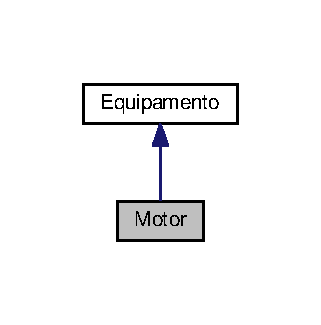
\includegraphics[width=154pt]{class_motor__inherit__graph}
\end{center}
\end{figure}


Collaboration diagram for Motor\+:
\nopagebreak
\begin{figure}[H]
\begin{center}
\leavevmode
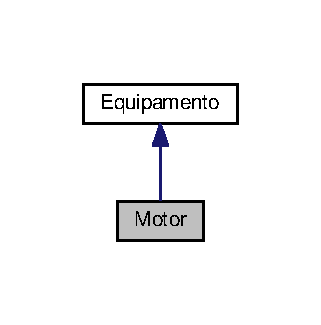
\includegraphics[width=154pt]{class_motor__coll__graph}
\end{center}
\end{figure}
\subsection*{Public Member Functions}
\begin{DoxyCompactItemize}
\item 
{\bfseries Motor} (int a=0)\hypertarget{class_motor_aa58ec792ec679b65913fec8619c5b9a2}{}\label{class_motor_aa58ec792ec679b65913fec8619c5b9a2}

\item 
void {\bfseries set\+Potencia} (float \+\_\+potencia)\hypertarget{class_motor_a9645ab1aa21f935db82717e047033d18}{}\label{class_motor_a9645ab1aa21f935db82717e047033d18}

\item 
void {\bfseries set\+Velocidade} (float \+\_\+velocidade)\hypertarget{class_motor_ac6abdb449f25131945ebe8c5a956445f}{}\label{class_motor_ac6abdb449f25131945ebe8c5a956445f}

\item 
float {\bfseries get\+Potencia} (void)\hypertarget{class_motor_a12bad50ec5ee50acaa9cfb1b63ab6726}{}\label{class_motor_a12bad50ec5ee50acaa9cfb1b63ab6726}

\item 
float {\bfseries get\+Velocidade} (void)\hypertarget{class_motor_a4da30fbd331875abe0cd1e158abdaf7c}{}\label{class_motor_a4da30fbd331875abe0cd1e158abdaf7c}

\item 
void {\bfseries set\+Preco} (float \+\_\+preco)\hypertarget{class_motor_ae13463bc31cba6521915af21b8bc01f9}{}\label{class_motor_ae13463bc31cba6521915af21b8bc01f9}

\end{DoxyCompactItemize}
\subsection*{Additional Inherited Members}


The documentation for this class was generated from the following files\+:\begin{DoxyCompactItemize}
\item 
motor.\+h\item 
motor.\+cpp\end{DoxyCompactItemize}

%--- End generated contents ---

% Index
\backmatter
\newpage
\phantomsection
\clearemptydoublepage
\addcontentsline{toc}{chapter}{Index}
\printindex

\end{document}
